\documentclass{article}
\usepackage[utf8]{inputenc}
\usepackage{geometry}
\usepackage{datetime2}
\usepackage{xparse}
\usepackage{amsmath}
\usepackage{booktabs}
\usepackage{array}
\usepackage{hyperref}


 \geometry{
 a4paper,
 total={170mm,257mm},
 left=20mm,
 top=20mm,
 }

 
 \usepackage{graphicx}
 \usepackage{titling}

 \title{Fuzzy Inference Untuk Paket Penjualan PV 
}
\date{18 March 2025}
 
 \usepackage{fancyhdr}
\fancypagestyle{plain}{%  the preset of fancyhdr 
    \fancyhf{} % clear all header and footer fields
    \fancyfoot[R]{}
    \fancyfoot[L]{}
    \fancyhead[L]{
\includegraphics[width=2cm]{ITS_pojok.pdf}}
    \fancyhead[R]{ \DTMnow}
}
\makeatletter
\def\@maketitle{%
  \newpage
  \null
  \vskip 1em%
  \begin{center}%
  \let \footnote \thanks
    {\LARGE \@title \par}%
    \vskip 1em%
    %{\large \@date}%
  \end{center}%
  \par
  \vskip 1em}
\makeatother

\usepackage{lipsum}  
% \usepackage{cmbright} % Change the font by zee

\begin{document}

\maketitle


\noindent\begin{tabular}{l @{ : } l}
        Nama                &  Septian Feter Arifianto \\  
        NIM                 &  6022251072 \\  
        Teacher             &  Muhammad Qomaruz Zaman, S.T., M.T., Ph.D.\\
        Mata Kuliah         &  Kecerdasan Buatan Assigment 3-Fuzzy Inference Untuk Paket Penjualan PV \\
\vspace{0,2cm}
        Class name          &  Kelas X\\
        GitHub Link & \url{https://github.com/septianfeter-arifianto/assigmet-3.git}\\
        Youtube & \url{https://youtu.be/ea4IYg5GnQI}\\
\end{tabular}
\vspace{1cm}

\section*{1. Pendahuluan}
Sistem ini digunakan untuk menentukan estimasi harga paket PV berdasarkan input luasan area dan daya (kWp) menggunakan metode Fuzzy Inference System.

\section*{2. Membership Function}
Parameter luasan menggunakan rentang skala 0 hingga 100 dengan tiga himpunan fungsi keanggotaan (Membership Function): 
\subsection*{2.1 Luasan PV}
\begin{itemize}
    \item Sedikit: Menjangkau nilai luasan dari 0 hingga batas 50.
    \item Sedang: Menjangkau rentang 0 hingga 100, dengan titik puncak berada pada nilai tengah 50.
    \item Banyak: Menjangkau nilai luasan dari batas 50 ke atas hingga 100.
       \begin{figure}[htbp]
    \centering
    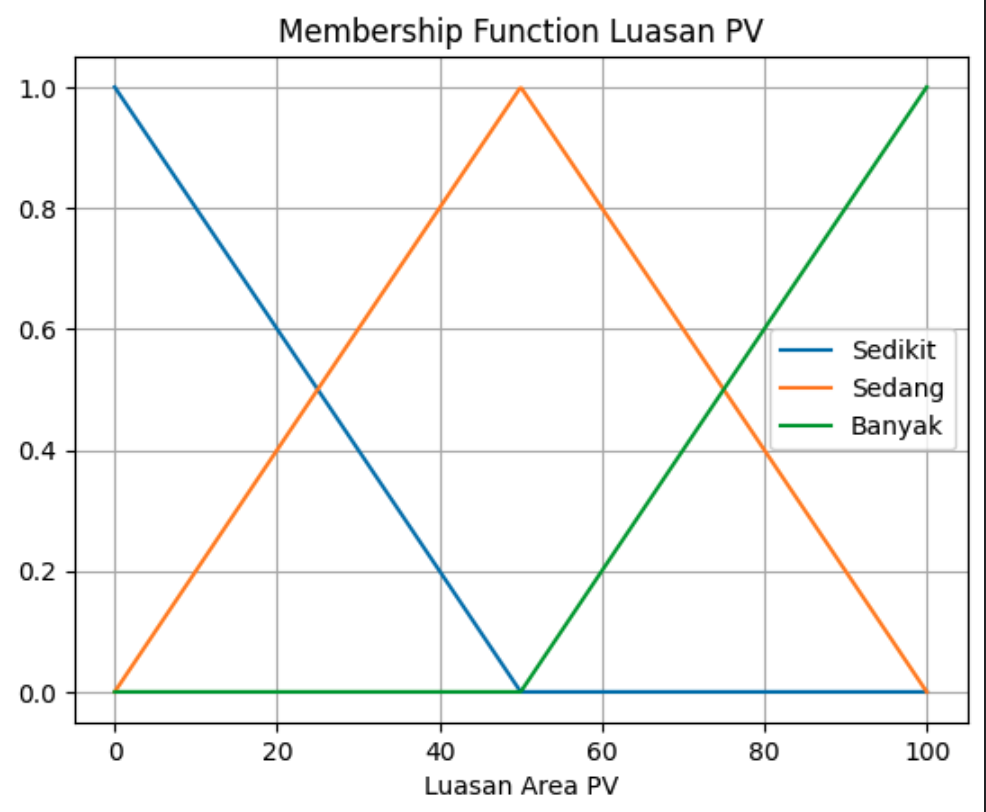
\includegraphics[width=0.5\linewidth]{Luas.png}
    \caption{Tabel}
    \label{fig:enter-label}
\end{figure}
\end{itemize}

\subsection*{2.2 Daya PV}
Parameter daya menggunakan rentang skala 0 hingga 10 dengan tiga himpunan fungsi keanggotaan.
\begin{itemize}
    \item Kecil: Menjangkau nilai daya dari 0 hingga batas 5.
    \item Menengah: Menjangkau rentang 0 hingga 10, dengan titik puncak berada pada nilai tengah 5.
    \item Besar: Menjangkau nilai daya dari batas 5 ke atas hingga 10.
    \begin{figure}[htbp]
    \centering
    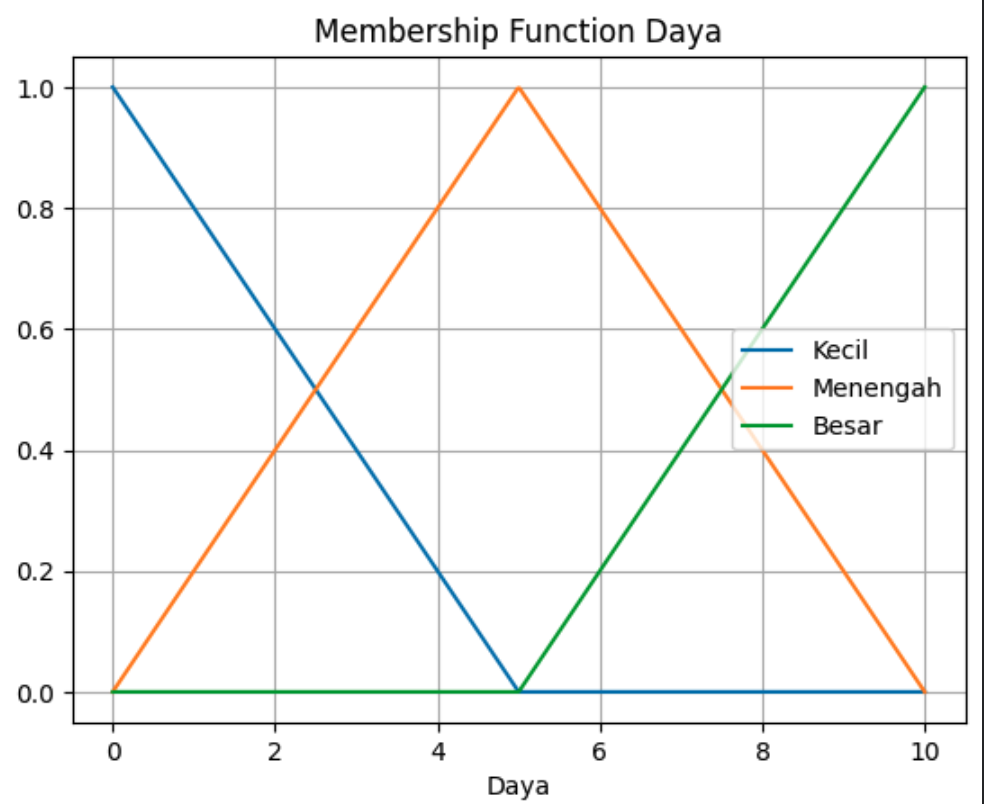
\includegraphics[width=0.5\linewidth]{Daya.png}
    \caption{Tabel}
    \label{fig:enter-label}
\end{figure}
\end{itemize}

\section*{3. Output Singleton}
Sistem ini menggunakan tiga kategori target keluaran (Z Output) berupa harga paket dengan nilai ketetapan (singleton) sebagai berikut:
\begin{itemize}
    \item Basic = 15
    \item Premium = 30
    \item Platinum = 50
\end{itemize}

\section*{4. Rule Base}
Berikut adalah matriks aturan yang ditetapkan untuk pengambilan keputusan pada sistem Fuzzy ini :
\begin{figure}[htbp]
    \centering
    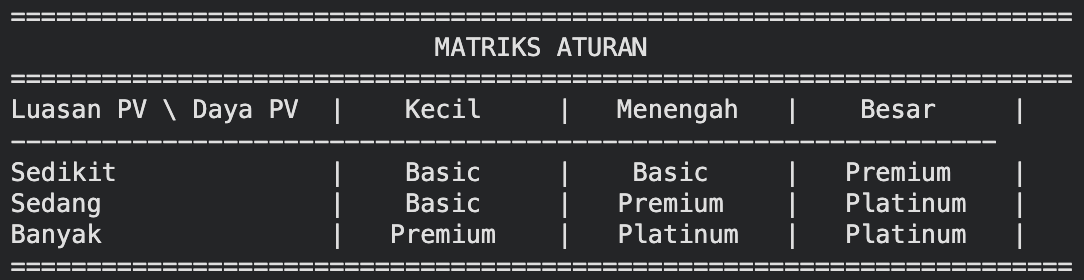
\includegraphics[width=0.5\linewidth]{Tabel.png}
    \caption{Tabel}
    \label{fig:enter-label}
\end{figure}

\section*{5. Penjelasan Rule}
\begin{itemize}
    \item Jika luasan PV sedikit dan daya kecil, maka digunakan paket Basic karena kapasitas kebutuhan secara keseluruhan merupakan yang paling minimal.
    \item Jika luasan PV sedikit namun daya besar, maka digunakan paket Premium untuk dapat mengakomodasi tingginya tarikan daya di lahan yang terbatas.
    \item Jika luasan PV sedang dan daya menengah, maka digunakan paket Premium sebagai bentuk titik seimbang kebutuhan standar.
    \item Jika luasan PV banyak dan daya besar, maka digunakan paket Platinum karena hal ini merepresentasikan spesifikasi tertinggi dari kapasitas energi PV.
\end{itemize}
\section*{6. Kesimpulan}
Metode Fuzzy Inference System dapat digunakan dengan efektif untuk mengevaluasi matriks aturan dan mengkalkulasi bobot rata-rata (Weighted Average) harga paket PV. Pada skrip pengujian, ketika diberikan input luasan 40 m² dan daya 6 kWp, sistem berhasil memproses hasil akhir dengan estimasi harga paket senilai Rp 30.71 Juta.
\end{document}


